\documentclass{article}

\usepackage{amsmath}
\usepackage[dvips]{graphicx}

\usepackage{natbib}

\bibliographystyle{apa}

\begin{document}

\title{Calibration of statistical classifiers\\
(working summary paper)}


\author{Peter Mills\\\text{peteymills@hotmail.com}}

\maketitle

\section{Background}

We are interested in maximum-likelihood statistical classifiers of the form:
\begin{equation}
	c(\vec x)=\max_j P(j|\vec x)
\end{equation}
where $c$ is the estimated class at test point $\vec x$ and
$P(j|\vec x)$ is the conditional probability of the class, $j$,
given $\vec x$.
Typically, $P(j|\vec x)$ is not known and we have only an estimate, 
lets call it $f_i(\vec x)$ or somewhat improperly, the {\it decision funciton}
(the term is normally only applied to binary classifiers).
How we arrive at $f$ is here immaterial. 
First, if probability estimates are available, or even if the decision function
does not estimate the probabilities, it may be used to recalibrate the class
estimates.
This recalibration need not always be done to improve accuracy but may have
other designs, for instance to minimize the number of false positives.
Moreover, there are many types of skill scores upon which to optimize.
Some of them will be discussed in this note.
Second, the decision function itself may be recalibrated based on
actual class values to better match actual probabilities.

\section{Classification skill}


The most common measure of classification skill, despite decades of progress
in the field, is still fraction or percentage of correct guesses, informally
called simply, ``accuracy''.
This is a poor skill measure for a number of reasons.
First, it will be affected by the composition of the test and training data.
For a binary classification problem in which 99\% of the data is ``true'',
you can get a 99\% accuracy simply by guessing true all the time.
This a 99\% accuracy means different things for different classification
problems.
There is another sense in which the score is not well calibrated.
A 0\% accuracy is not the worst skill score.
The worse accuracy would be $1/n_c$ where $n_c$ is the number of class labels
since this would be expected by random chance.
On the contrary, 0\% accuracy is a very good score since it cannot be 
expected by random chance (except on very small problems).
Rather the classifier is guessing consistently, it's just that the labels
have been rearranged.

\subsection{Uncertainty coefficient}

A skill score that eliminates these problems is the uncertainty coefficient
which measures how many bits on average the classifier conveys per result of the
actual class value.
It is based on information entropy:
\begin{equation}
	H_i=-\sum_i p_i \log p_i
\end{equation}
where $H$ is the entropy and $p_i$ is a discrete probability.
Let $p_{ij}$ be the joint probability of class $i$ and class $j$
and $p(i|j)$ be the conditional probability of class $i$ given $j$.
The conditional entropy is given:
\begin{equation}
	H(i|j)=-\sum_i p_{ij} \log p(i|j)
\end{equation}
The uncertainty coefficient is defined as the channel capacity normalized
by the input distribution:
\begin{equation}
	U=\frac{H_i - H(i|j)}{H_i}
\end{equation}
This measure has the dual advantage that it is not affected by the relative sizes
of the classes nor does it penalize mis-labelling: so long as a classifier
does so consistently, rearranging the class labels does not affect the 
score.
Here we can think of class $i$ as the ``truth'' and $j$ as the estimated
class, however a symmetric measure can be defined by forming a weighted 
combination of both the forward and reverse measures:
\begin{eqnarray}
	H(i,j)&=&\frac{H_i U(i|j) + H_j H(j|i)}{H_i + H_j}\\
	      &=&2\left [\frac{H_i + H_j - H_{ij}}{H_i + H_j} \right ]
\end{eqnarray}
where the joint entropy, $H_{ij}$, is given:
\begin{equation}
	H(i|j)=-\sum_i p_{ij} \log p_{ij}
\end{equation}

\subsection{Confusion matrix}

The most comprehensive measure of classification skill, and the one upon
which all the others are built, is the {\it confusion matrix}, although
it needs some interpretation to be useful.
Here is an example of a confusion matrix:
\begin{verbatim}
        retrieval
truth    0    1    2    3    4    5    6    7    8    9     tot
  0    352    0    0    0    0    0    0    0   11    0     363
  1      0  351    8    2    1    0    0    2    0    0     364
  2      0    2  362    0    0    0    0    0    0    0     364
  3      0    1    0  333    0    0    0    0    0    2     336
  4      0    0    0    0  358    5    1    0    0    0     364
  5      0    0    0    3    0  330    0    0    1    1     335
  6      0    0    0    0    0    0  336    0    0    0     336
  7      0    8    2    2    0    0    1  339    0   12     364
  8      2    0    0    0    0    1    0    0  333    0     336
  9      0    1    0    1    0    2    0    3    1  328     336

total  354  363  372  341  359  338  338  344  346  343
\end{verbatim}
Let $n_{ij}$ be the element on the $i$th row and $j$th column of the matrix
which tells us: for each value of the $i$th class, how many results of the
$j$th class does the classifier return?
Thus the accuracy is given:
\begin{eqnarray}
	a&=&\frac{\sum_i n_{ii}}{\sum_{i,j} n_{ij}}\\
	 &=&\mathrm{tr}{N}/n_t
\end{eqnarray}
where $N=\lbrace n_{ij} \rbrace$ is the whole confusion matrix and
$n_t$ are the total number of classification results in the matrix.
Similarly, we approximate $p_{ij}$ in the calculation of the uncertainty
coefficient:
\begin{equation}
	p_{ij}\approx n_{ij}/n_t
\end{equation}

\subsection{Binary skill scores}

The confusion matrix for a binary classifier has only four elements:
\begin{equation}
	N = \left ( \begin{array}{cc}
		n_{TN} & n_{FP} \\
		n_{FN} & n_{TP}
	\end{array} \right )
\end{equation}
where $n_{TN}$ is the number of true negatives, $n_{FN}$ is the number of
false negative, $n_{FP}$ is the number of false positives and $n_{TP}$ is
the number of true positives.
Despite the apparent simplicity, there are still a surprising diversity of
different skill scores that can be constructed from just these four elements:
see for instance \citet{Jolliffe_Stephenson2003}.
Here we show just one--the correlation coefficient \citep{Mills2004}:
\begin{equation}
	r = \frac{n_{TN} n_{TN} - n_{FN} n_{FP}}
	{\sqrt{(n_{TP}+n_{FP})(n_{TN}+n_{FN})(n_{TP}+n_{FN})(n_{FP}+n_{TN})}}
\end{equation}
which, like the uncertainty coefficient, has the advantage of being well-
calibrated except that it will inform you of a mis-labelling error by returning
a negative value.


\section{Calibrating binary classifiers}

\subsection{Definitions}

We summarize the result of a binary classification using a single variable, 
$r \in [-1, ~1]$, the difference in conditional probabilities:
\begin{equation}
	r(\vec x) \approx P(2|\vec x) - P(1|\vec x)
\end{equation}
For a maximum
likelihood classification, we choose the threshold value for $r$, $r_0$,
that discriminates between the two classes,
\begin{equation}
c = \left \lbrace
\begin{array}{lr}
1 & r<r_0 \\
2 & r>r_0
\end{array}
\right .
\end{equation}
as $r_0 = 0$, but there is no reason why this should be so.  
In both \citet{Mills2009} and \citet{Mills2011}, we show how shifting this
border can be used to recalibrate an image derived from statistical
classification.

This threshold is equivalent to both a constant value for the conditional
probabilities:
\begin{eqnarray}
r_0 & = & p_2 - p_1 \\
& = & 1 - 2 p_1
\end{eqnarray}
as well as a ratio:
\begin{eqnarray}
f & = & \frac{p_2}{p_1} \\
  & = & \frac{1 - p_1}{p_1}
\end{eqnarray}
Solving for $p_1$ and equating the two produces the following:\
\begin{eqnarray}
p_1 & = & \frac{1}{f+1} = \frac{1 - r_0}{2} \\
r_0 & = & \frac{f-1}{f+1} \\
f & = & \frac{1+r_0}{1-r_0}
\end{eqnarray}

\subsection{Correcting for class size}

Shifting the threshold can also be used to correct for the case in which we
are training the model using a set of samples whose class statistics
differ from those of the population.
Let $P(1)$ and $P(2)$ be the relative class numbers of the population while
$P^\prime(1)$ and $P^\prime(2)$ are the class numbers of the sample.
Typically, we want:
\begin{equation}
r=P(2|\vec x)-P(1|\vec x)=
\frac{P(2)P(\vec x|2)}{P(\vec x)}-\frac{P(1)P(\vec x|1)}{P(\vec x)} = 0
\end{equation}
or:
\begin{equation}
\frac{P(\vec x|1)}{P(\vec x|2}=\frac{P(2)}{P(1)}
\end{equation}
We want to find an $f$ such that the sample statistics are corrected to
the populations statistics:
\begin{equation}
f = \frac{P^\prime(2)P(\vec x|2)}{P^\prime(1)P(\vec x|1)}
=\frac{P^\prime(2) P(1)}{P^\prime(1) P(2)}
\end{equation}
or:
\begin{equation}
r_0=\frac{P^\prime(2)P(1) - P^\prime(1) P(2)}
	{P^\prime(2)P(1) + P^\prime(1)P(2)}
\end{equation}

\begin{figure}
\includegraphics[width=0.9\textwidth,angle=-90]{rhist.eps}
\caption{Cumulative distribution function (axes reversed) 
of the difference in conditional
probabilities, $r=P(2|\vec x)-P(1|\vec x)$
for the pair of sample classes described in \citet{Mills2011}.}
\label{rhist}
\end{figure}

\begin{figure}
\includegraphics[width=0.9\textwidth,angle=-90]{skillvsr0.eps}
\caption{Two skill scores, accuracy and uncertainty coefficient, as a function of
the decision threshold, $r_0$,
for the pair of sample classes described in \citet{Mills2011}.}
\label{skillvsr0}
\end{figure}

\begin{figure}
\includegraphics[width=0.9\textwidth,angle=-90]{sample_roc.eps}
Receiver operating characteristic (ROC) curve
for the pair of sample classes described in \citet{Mills2011}.
\label{sample_roc}
\end{figure}

\subsection{Shifting the discrimination border}

In binary classification, the discrimination border can be shifted so as to
optimize any desired skill score.  Since only one parameter is being varied,
the optimization is a straightforward numerical procedure.  Any numerical
minimization technique, such as golden section search \citep{Press_etal1992},
that doesn't require derivatives (which will be discontinuous), can be used.

Figure \ref{rhist} shows the cumulative distribution,
$r$, $F(r)$ for the sample classes discussed in \citet{Mills2011}.  
From this, we can in theory
calculate any skill score for a binary classifier we desire, since:
\begin{eqnarray}
\frac{n_{TP}}{n} & = & \frac{1}{2}\int_{r_0}^{1} (r+1) 
		\frac{\mathrm d F}{\mathrm d r} \mathrm d r \\
		& = & F(1) - F(r_0) + 
		\int_{r_0}^{1} F r \mathrm d r - \int_{r_0}^{1} F \mathrm d r \\
		& = & 1 - F(r_0) + \int_{r_0}^{1} F r \mathrm d r - \int_{r_0}^{1} F \mathrm d r \\
\frac{n_{FP}}{n} & = & \frac{1}{2}\int_{r_0}^{1} (1-r) 
		\frac{\mathrm d F}{\mathrm d r} \mathrm d r \\
		& = & 1 - F(r_0) - 
		\int_{r_0}^{1} F r \mathrm d r + \int_{r_0}^{1} F \mathrm d r \\
\frac{n_{TN}}{n} & = & \frac{1}{2}\int_{-1}^{r_0} (1-r) 
		\frac{\mathrm d F}{\mathrm d r} \mathrm d r \\
	& = & F(r_0) - F(-1) -
		\int_{-1}^{r_0} F r \mathrm d r + \int_{-1}^{r_0} F \mathrm d r \\
	& = & F(r_0) - \int_{-1}^{r_0} F r \mathrm d r + \int_{-1}^{r_0} F \mathrm d r \\
\frac{n_{TP}}{n} & = & \frac{1}{2}\int_{-1}^{r_0} (r+1) 
		\frac{\mathrm d F}{\mathrm d r} \mathrm d r \\
	& = & F(r_0) + \int_{-1}^{r_0} F r \mathrm d r - \int_{-1}^{r_0} F \mathrm d r 
\end{eqnarray}
where $n_{TP}$, $n_{FP}$, $n_{TN}$, and $n_{FN}$ are the number of true positives
, false positive, true negative and false negatives, respectively, and $n$
is the total number of classes.

The conditional probabilities are calculated based on the definitions of the
probability functions as described in \citet{Mills2011}.  For simple
accuracy, that is, fraction of correct predictions, the optimal decision
threshold should, if the probabilities are estimated accurately,
lie close to zero.
For the uncertainty coefficient, which measures the
number of bits of information contained in each prediction
\citep{Shannon, Press_etal1992, Mills2011}, changing the location of the
decision threshold can considerably improve skill scores.  In particular,
if one class is larger than the other, moving the decision border 
{\it closer} to it will typically improve the uncertainty coefficient.
These results are summarized in figure \ref{skillvsr0}.

Presumably, if the classes have been re-calibrated, then the associated 
conditional probabilities need to be transformed also.
Consider the following two transformations:
\begin{equation}
r^\prime = \left \lbrace
\begin{array}{lr}
\frac{r-r_0}{1-r_0} & r<r_0 \\
\frac{r_0-r}{r_0+1} & r>r_0
\end{array} \right \rbrace
\end{equation}
and:
\begin{equation}
r^\prime=\tanh \left (\tanh^{-1}(r)-\tanh^{-1}(r_0) \right ]
\end{equation}
with the second version being similar to what happens after setting the 
\verb/-r/ switch using \verb/class_borders/ in the {\it libagf} package.
Both these have the nice property both that transformed probabilities sum
to one and, if the original probability is one, then so are the transformed
probabilities:
\begin{equation}
p_i^\prime=1 \iff p_i=1
\label{ptop}
\end{equation}

\subsection{ROC curve}

The parameter, $r_0$, can also be used to construct 
the receiver operating characteristic (ROC) curve \citep{Jolliffe_Stephenson2003}.
This is the hit rate:
\begin{equation}
	H = \frac{n_{TP}}{n_{FN} + n_{TP}}
\end{equation}
plotted against the false alarm rate:
\begin{equation}
	F = \frac{n_{FP}}{n_{FP} + n_{TN}}
\end{equation}
The ROC curve for the pair of sample classes is shown in figure
\ref{sample_roc}.
Integrating the area under the ROC curve will produce a calibration-independent
skill score:
\begin{equation}
	A = \int_0^1 H(F) \mathrm d F
\end{equation}
[how would one do this for a parametric curve, $H(r_0)$, $F(r_0)$ ?]
A perfect score would be 1: the curve goes straight up from the origin
until it hits 1, then runs horizontal until it hits (1,1).
The worst possible outcome would be the diagonal line for, $A=0.5$.
Mis-labeled systems would fall below the diagonal.

\section{Calibrating the probabilities}

Sometimes we are interested in the accuracy of the probabilities themselves.
Suppose $P(j|\vec x)$ is equal to 0.6 for instance, then we would expect
that the actual class, $c(\vec x)$, would be equal to $j$ 60\% of the time.
This means gathering enough instances where $P(j|\vec x)=0.6$ to produce
useful statistics.
An obvious approach is binning: divide the probabilities into ranges.
Statistics of actual class ratios are gathered within each range of the estimated
probabilities and compared with averages of the estimated probabilities.


\bibliography{../agf_bib.bib} 

\end{document}
